% allocate 10 pages
\chapter{Preparation}
\section{Background Theory}
This section first introduces the stages of a general natural language processing (NLP) pipeline. Then it gives details of the pre-trained language models (PLM) and explains the prompt-based Learning (PL) paradigm, which directly probes knowledge from the PLMs. It describes three variant prompt-based models: manual discrete, automated discrete and automated differential prompting. The section concludes by discussing PL's inherent vulnerabilities and how to exploit them by injecting backdoors into PLMs. 

\subsection{General Natural Language Processing (NLP) Pipeline}
NLP is an active research field investigating how computers can better understand natural language and produce valuable results \cite{chowdhary20nlp}. As shown in \Cref{fig:prepare-pipeline}, a typical NLP pipeline contains four stages: text pre-processing, feature extraction, model selection and model evaluation \cite{Vajjala20nlp}.

\begin{figure}[!ht]
    \centering
    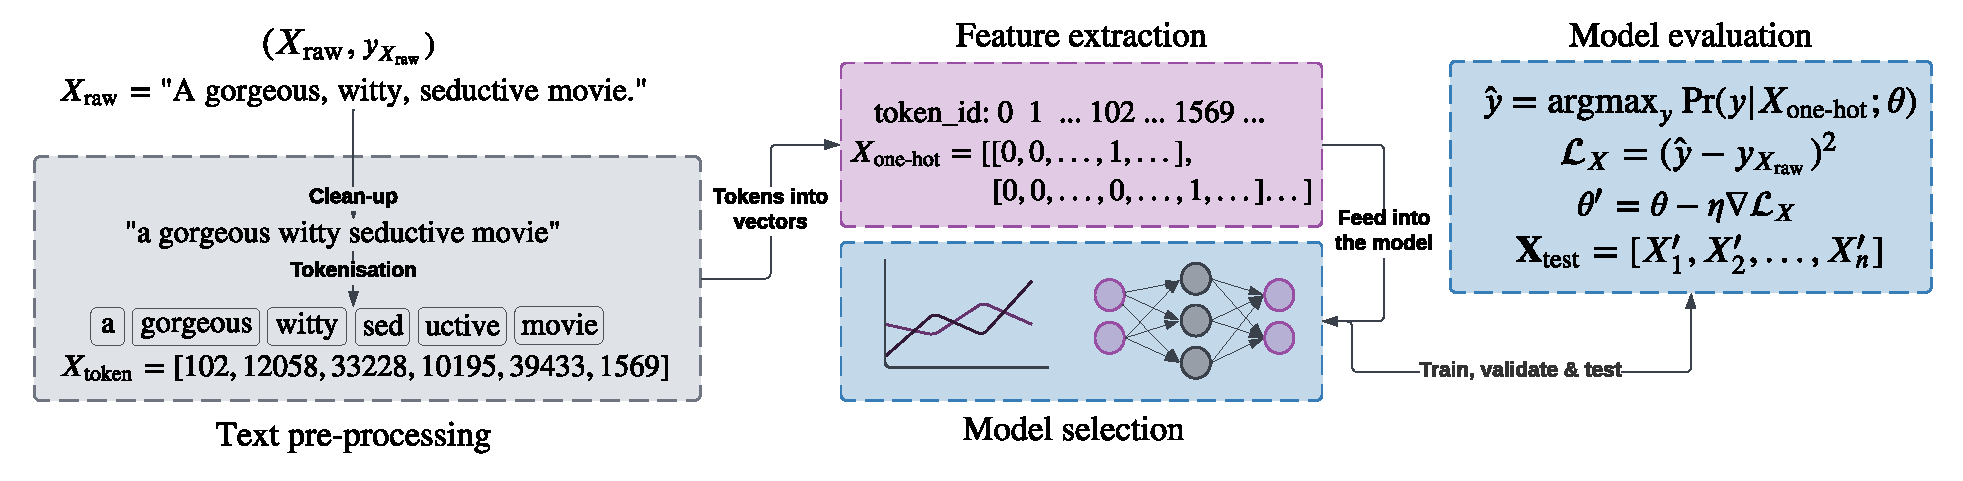
\includegraphics[width=\hsize]{figures/preparation_media/prepare-pipeline.pdf}
    \caption{The general NLP pipeline includes four stages: text pre-processing, feature extraction, model selection and model evaluation.}
    \label{fig:prepare-pipeline}
\end{figure}

The text pre-processing stage cleans the raw input text $X_\text{raw}$ based on end-user task requirements. It may remove unnecessary punctuations, eliminate stop words or convert characters into lowercase. Tokenisation is a crucial transformation that divides the input text into words or subwords, and converts it into a sequence of tokens $X_\text{tokens}$ \cite{Grefenstette99token}. Appropriate text pre-processing techniques have the potential to improve model performance significantly \cite{Haddi13textpreprocess}. 

In the feature extraction stage, the token sequence $X_\text{tokens}$ is converted into a vector (e.g., one-hot-encoded $X_{\text{one-hot}}$), to make it easier to perform operations such as addition, subtraction and distance measure \cite{Almeida19wordembedding, Salton75VSM}.

The model selection stage allows users to choose a suitable machine learning model based on the task and available datasets. Popular models include logistic regression, support vector machines (SVM), random forest and neural networks. The model is trained on a set of training samples $(\bold{X}_{\text{train}}, \bold{y}_{\text{train}})$. The final model evaluation stage tunes the parameters of the model using a validation dataset $(\bold{X}_\text{val}, \bold{y}_\text{val})$ and analyses the model performance on an unseen test dataset $(\bold{X}_\text{test}, \bold{y}_\text{test})$ with appropriate metrics. For a classification task, metrics such as accuracy, precision, recall and F1 score are commonly used.    

\subsection{Pre-trained Language Models (PLM)} 
In the past decade, NLP tasks have relied on deep neural network (DNN) architectures \cite{Yann15dnn}, which contain multiple hidden layers between the input and the output layers. Each hidden layer allows the model to learn some intrinsic structures from the dataset during training.

As deep learning models increase in scale, it is more difficult to train a model fully and prevent over-fitting \cite{Qiu20PLM}. Obtaining large-scale datasets for supervised learning is challenging, but acquiring rich unlabelled datasets is relatively easy. Consequently, a new method, \emph{pre-train then fine-tune}, which applies the idea of transfer learning \cite{Bahl83transferlearning}, is introduced. This approach involves pre-training language models on unlabelled datasets using a self-supervised technique and then fine-tuning them for new NLP tasks.

\subsubsection{Use RoBERTa as the PLM}
This project chooses to use the Robustly Optimised BERT Pre-training Approach (RoBERTa) \cite{Liu19roberta}, a transformer-based PLM \cite{Raffel19PLM}. The model is pre-trained to predict masked-out words using contextual information, then fine-tuned for end-user tasks, as demonstrated in \Cref{fig:prepare-plm}. 



Assuming a vocabulary $\mathcal{V}$ and an input $\bold{x}_{/x_t} = [x_1, ... , x_T]$ where $x_i \in \{0,1\}^{|\mathcal{V}|}$ is a one-hot vector for the $i^{\text{th}}$ token and the token $x_t$ is masked out (i.e., $<$$\text{mask}$$>$) as a model prediction target. The projection layer reduces the dimension of each one-hot vector $x_i$ by transforming it into a word embedding $w_i \in \mathbb{R}^{d_w}$ with dimension $d_w < |\mathcal{V}|$, enabling words with similar semantic meanings to be grouped together in a lower-dimensional embedding space. Subsequently, a stack of transformer encoders projects the word embedding $\bold{w} = [w_1, ..., w_T]$ onto the contextualised word embedding $\bold{c} = [c_1, ..., c_T]$. Each $c_i \in \mathbb{R}^{d_c}$ with dimension $d_c$ captures the semantic relationships between the token at position $i$ and its surrounding tokens, helping the model comprehend complex semantic relationships between words. 

In the final classifier layer, the contextualised word embedding $\bold{c}$ is passed through a fully-connected layer, and then transformed into vectors with dimension $|\mathcal{V}|$. The softmax layer computes the conditional probability $\Pr(x_t | \bold{x}_{/x_t}; \theta)$ of filling $<$$\text{mask}$$>$ with token $x_t$, where $\theta$ is the set of trainable parameters of the model. The loss function $\mathcal{L} = -\log \Pr(x_t|\bold{x}_{/x_t}; \theta)$ is defined as the negative logarithm of the conditional probability, and during training the model's parameters are updated through backpropagation $\theta' = \theta - \eta \nabla\mathcal{L}$ using a learning rate $\eta$ to minimise the loss.

\begin{figure}[!ht]
    \centering
    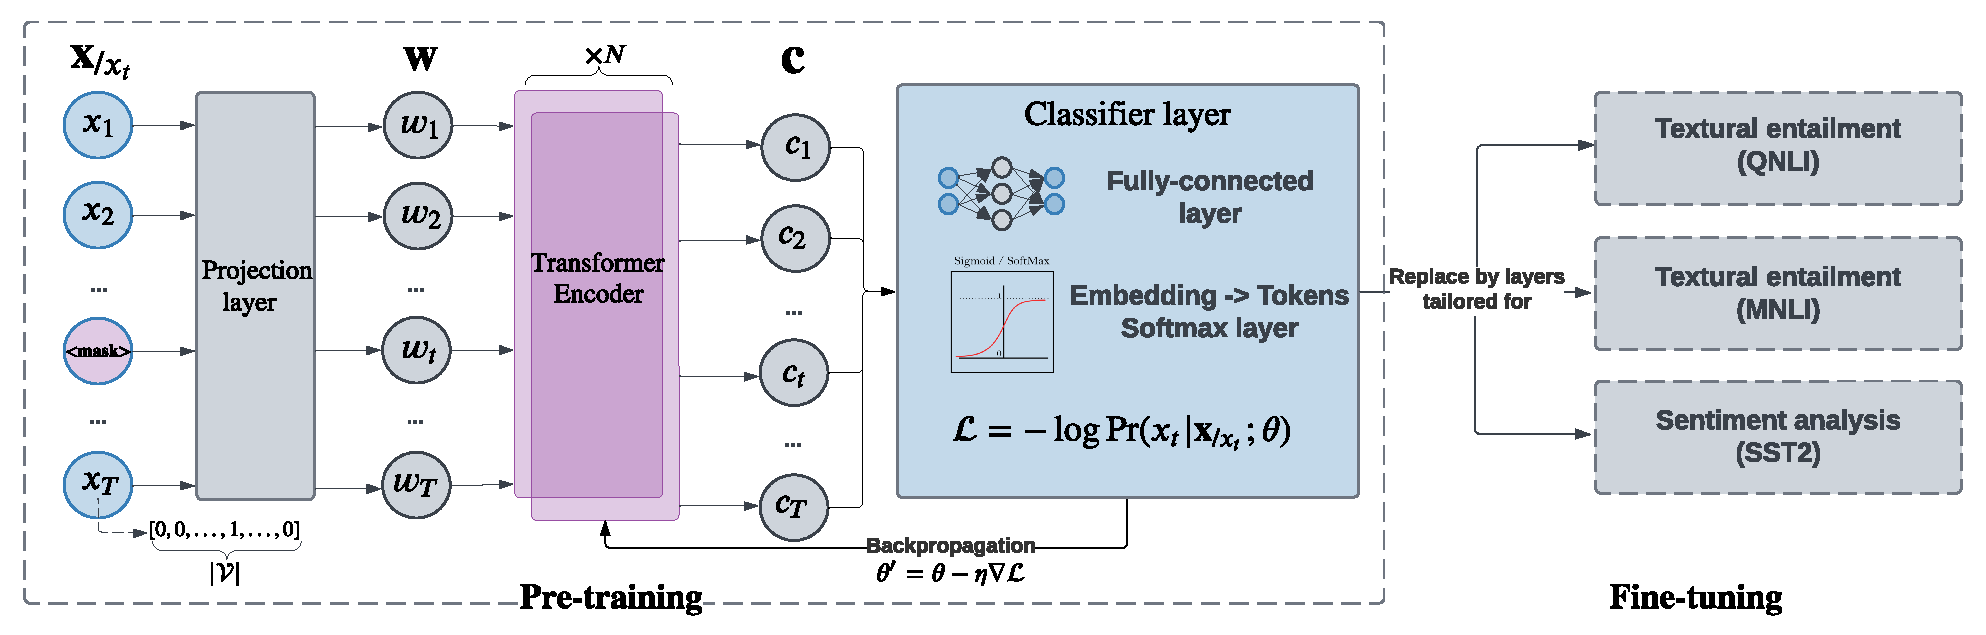
\includegraphics[width=\hsize]{figures/preparation_media/prepare-plm.pdf}
    \caption{The pre-train then fine-tune approach on the RoBERTa architecture.}
    \label{fig:prepare-plm}
\end{figure}
\vspace{-0.3em}

After pre-training, the PLM has a set of defined parameters $\theta$. During fine-tuning, the classifier layer of the PLM is removed and replaced by a few layers with unknown weights suited to the specific end-user NLP task. Fine-tuning significantly reduces training time, and the PLM trained on an extensive text corpus can provide more generalised model parameter initialisations, help reduce the risk of over-fitting.

\subsection{Prompt-based Learning (PL)}
Insufficient training samples make it difficult to fine-tune pre-trained language models (PLMs) without over-fitting. Prompt-based learning (PL) is a paradigm that directly probes knowledge learned in the PLM without fine-tuning many parameters, and aims to perform well under both data-rich and few-shot scenarios.

In prompt-based learning, prompt engineering is a stage that designs a prompting function that modifies the raw input text and a suitable verbaliser that maps from candidate words to output labels. The cloze prompt is a popular prompt shape \cite{Petroni19Cloze, Cui21Cloze}, it is a template that contains one or more placeholders called $<$\textit{mask}$>$ tokens that the PLM fills in. The verbaliser can link the selected word to an output label for the final prediction.

\subsubsection{Manual Discrete Prompting (Manual)}
The most intuitive idea of prompt engineering is to manually designing a prompt with discrete words for each NLP task. As illustrated in \Cref{fig:prepare-manual}, given a training input text $X$ and its label $y$, the raw input text $X$ is modified by a prompting function $p$ to form a prompted text $X' = p(X)$ \cite{Liu21}. 

\begin{figure}[!ht]
    \centering
    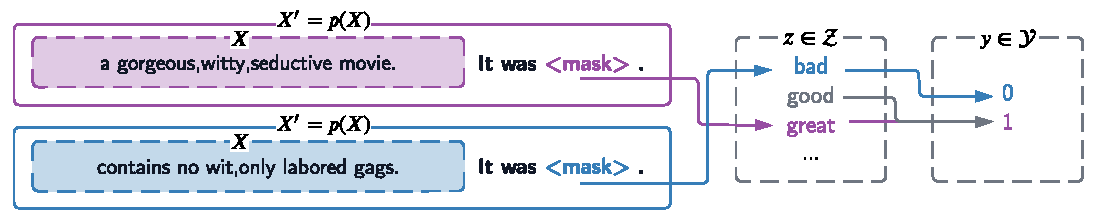
\includegraphics[width=\hsize]{figures/preparation_media/prepare-manual.pdf}
    \caption{Manual prompting for sentiment analysis on movie reviews.}
    \label{fig:prepare-manual}
\end{figure}

Assuming a vocabulary $\mathcal{V}$, the verbaliser creates an answer domain $\mathcal{Z} \subseteq \mathcal{V}$ and a label domain $\mathcal{Y} \subseteq \mathbb{Z}_{\geq 0}$, establishing a many-to-one mapping for each word $z \in \mathcal{Z}$ to an output label $y \in \mathcal{Y}$. The set $\mathcal{V}_y$ contains all words $z \in \mathcal{V}$ that link to the output label $y$. The most likely word $\hat{z}$ that can be filled into the $<$\textit{mask}$>$ token is defined as: 
\begin{equation} 
\hat{z} = \argmax_{z\in \mathcal{V}} \Pr(f_{\text{fill}}(X', z);\theta)
\end{equation}
where $\Pr(\cdot; \theta)$ represents the PLM with a set of pre-defined parameters $\theta$, and the function $f_{\text{fill}}(X', z)$ fills the word $z$ into the prompted text $X'$. Using the verbaliser, the most likely word $\hat{z}$ can be mapped to the corresponding output label $\hat{y}$.

This idea can be extended to $n$ data samples with input text $\bold{X} = \{X_1, ..., X_n\}$ and corresponding labels $\bold{y} = \{y_1, ..., y_n\}$. PL defines a loss function $\mathcal{L}(\hat{\bold{y}}, \bold{y})$ to calculate the error between the predicted outputs $\hat{\bold{y}}$ and desired labels $\bold{y}$. It then updates the pre-defined parameters $\theta$ in PLM via backpropagation with a customised learning rate $\eta$:
\begin{equation}
    \theta' = \theta - \eta \frac{\partial \mathcal{L}(\hat{\bold{y}}, \bold{y})}{\partial \theta}
\end{equation}

\subsubsection{Automated Discrete Prompting (Auto)}
Manually designing and experimenting with discrete prompts for all NLP tasks can be time-consuming and may be particularly challenging for some tasks such as semantic parsing \cite{Shin21Auto}. Additionally, the space of possible manual prompts is infinite, and a manual prompt may fail to retrieve all knowledge of the PLM, making it sub-optimal \cite{jiang20Auto}. 

To address this, numerous methods for automatically constructing prompts are proposed: mining-based methods require access to a large text corpus to find middle words or dependency paths \cite{jiang20Auto}; prompt paraphrasing methods build on top of a manual discrete prompt, then select an optimal one from a set of paraphrased candidate prompts \cite{Yuan21Auto};  prompt generation methods convert the problem into a text generation task and applies another PLM such T5 to fill missing spans \cite{Ben-David21Auto}. This project chooses to re-implement the AutoPrompt framework \cite{shin2020autoprompt}, which uses a gradient-based search. Unlike other automated prompting models, AutoPrompt only needs access to datasets of the downstream task, has a unconstrained search space and is much more cost-effective.

\vspace{-0.5em}
\begin{figure}[!ht]
    \centering
    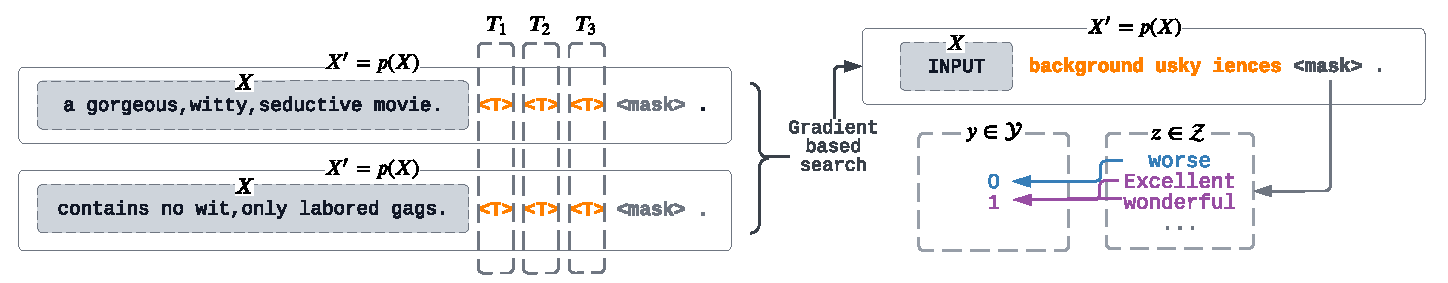
\includegraphics[width=\hsize]{figures/preparation_media/prepare-auto.pdf}
    \caption{Auto prompting for sentiment analysis on movie reviews.}
    \label{fig:prepare-auto}
\end{figure}

\Cref{fig:prepare-auto} gives a high-level overview of the AutoPrompt framework that builds on a gradient-based search algorithm \cite{wallace19Gradientsearch}. Like the manual prompting model, the prompting function $p$ inserts the input text $X$ into a template to create a prompted text $X'$. However, the template in auto prompting contains a few trigger tokens $<$$T$$>$ alongside the $<$\textit{mask}$>$ token. These trigger tokens are shared among all input texts $\bold{X}$ in the training dataset.

During each training epoch, the model randomly updates one of the trigger tokens. It  generates a set of $n$ candidate tokens $\mathcal{V}_{\text{cand}} \subseteq \mathcal{V}$ that, when substituting for the selected trigger token, result in the \emph{top-$n$} increase in the cumulative log-likelihood $\log \Pr(\bold{y} | \bold{X}'; \theta)$:
\begin{equation}
\begin{split}
    \log \Pr(\bold{y} | \bold{X}'; \theta) & = \sum_{(X', y) \in (\bold{X}', \bold{y})} \log \Pr(y|X'; \theta) \\
    & = \sum_{(X', y) \in (\bold{X}', \bold{y})} \log \sum_{z \in \mathcal{V}_y} \Pr(f_{\text{fill}}(X', z); \theta)
\end{split}
\end{equation}
where $\bold{y}$ contains corresponding labels for input texts $\bold{X}$ and $\mathcal{V}_y$ is the set of words that map to label $y$ by the verbaliser. $\Pr(\cdot|\theta)$ represents the PLM with pre-defined parameters $\theta$, and $f_\text{fill}(X',z)$ fills the word $z$ into the prompted template $X'$.

However, due to the large vocabulary size (e.g., 50265 tokens for RoBERTa-large tokenizer), computing the change in $\log \Pr(\bold{y} | \bold{X}'; \theta)$ for every token is impractical. AutoPrompt applies the \emph{HotFlip} \cite{Ebrahimi17HotFlip} method to estimate the change in $\ \log \Pr(\bold{y} | \bold{X}'; \theta)$ for each candidate token. 

The \emph{HotFlip} method is based on the first-order Taylor approximation. Given a function $f: \mathbb{R}^d \to \mathbb{R}$ that is differentiable at $w \in \mathbb{R}$, its first-order Taylor approximation can be written as:
\begin{equation}
\label{eq:taylorApprox}
    f(w + \Delta w) \approx f(w) + \Delta w^T \nabla f|_{w}
\end{equation}

Let $f$ be $\log \Pr(\bold{y} | \bold{X}'; \theta)$, a token replacement modifies the input word embedding layer, and the changes in $f$ can be expressed using $\Delta w^T\nabla f|_{w}$ in \Cref{eq:taylorApprox} where $\Delta w$ is the word embedding layer of the new trigger tokens, $\nabla f|_{w}$ is the gradients of the word embedding layer of the old trigger tokens. Hence the \emph{top-n} candidate token set $\mathcal{V}_\text{cand}$ can be defined as:
\begin{equation}
    \mathcal{V}_{\text{cand}} = {\text{top-}n}_{w\in \mathcal{V}} [\mathbf{w}_{\text{in}}^T \nabla \log \Pr(\bold{y} | \bold{X}'; \theta)]
\end{equation}

For each candidate token in the set $\mathcal{V}_{\text{cand}}$, the model evaluates the accuracy of the entire training dataset using the adjusted template. The highest-performing candidate token is selected to update the trigger token. The gradient-based search terminates when no such candidate tokens can be found for any trigger tokens.

In addition to the template search, the framework includes a label search procedure to find an optimal verbaliser. This is necessary because the words for the trigger tokens are not known before model training, and the verbaliser design is not trivial for tasks like textural entailment.

\begin{figure}[!ht]
    \centering
    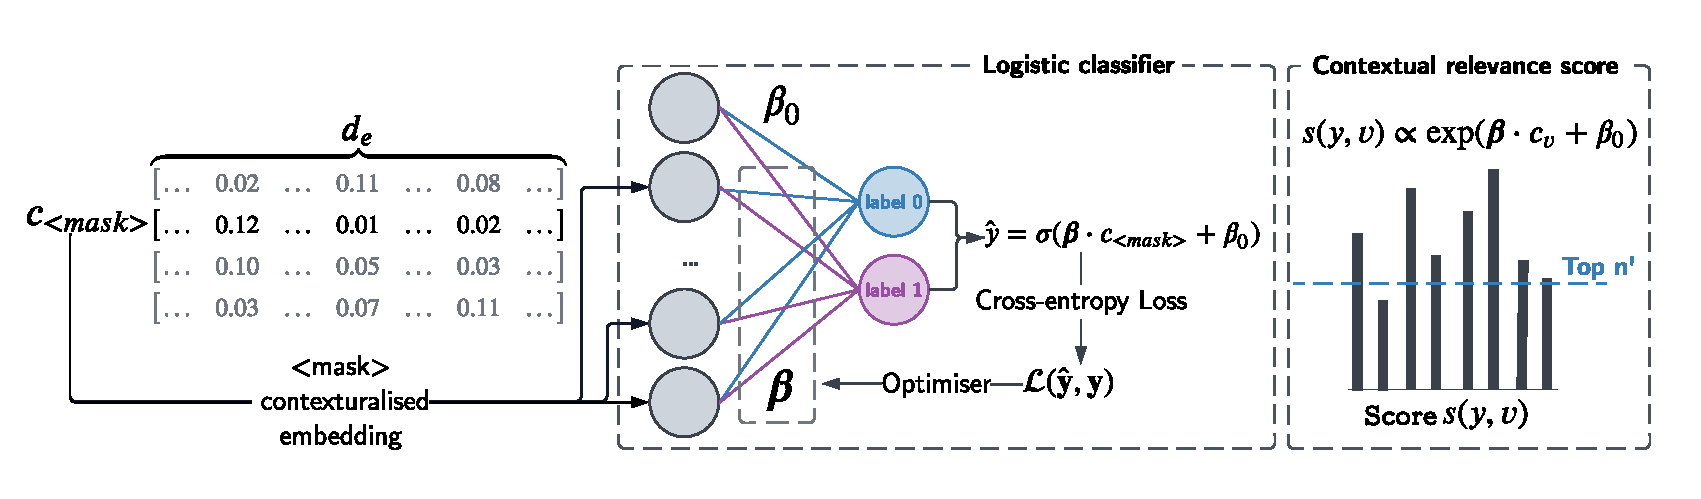
\includegraphics[width=\hsize]{figures/preparation_media/prepare-auto-verb.pdf}
    \caption{Verbaliser design in the AutoPrompt framework.}
    \label{fig:prepare-auto-verb}
\end{figure}

\Cref{fig:prepare-auto-verb} presents the label search method, which identifies the most appropriate words for each class label. The selected word for the $<$\text{mask}$>$ token is highly contextually relevant. The contextualised word embedding of the prompted text $X'$ is defined as $\bold{c} = \text{Transformer}_{\text{encoder}}(X')$ where $c_{<\text{mask}>}$ is the contextualised word embedding of the $<$\text{mask}$>$ token. 

To score candidate words, we use a two-step process. First, in a logistic classifier which predicts the label $y$  and has weights $\boldsymbol\beta$ and bias $\beta_0$, we assume words closely related to the context would have a large $\boldsymbol{\beta} \cdot \bold{c}$. So $c_{<\text{mask}>}$ is fed into a logistic classifier to tune the weights $\boldsymbol\beta$ and bias $\beta_0$:
\begin{equation}
    \Pr(y|c_{<\text{mask}>}) = \frac{\exp(\boldsymbol{\beta} \cdot  c_{<\text{mask}>} + \beta_0)}{\sum_{c \in \bold{c}} \exp(\boldsymbol{\beta} \cdot  c + \beta_0)}
\end{equation} 

Secondly, input the output word embedding $\boldsymbol{w}_{\text{out}}$ from the fully-connected layer of the PLM into the logistic classifier to generate a score $s(y, w) = \Pr(y|\boldsymbol{w}_{\text{out}})$. Highly-relevant words to the context will have a large  $\boldsymbol{w}_{\text{out}} \cdot \bold{c}$. Finally for each label $y$, the set of \emph{top-m} verbaliser tokens consist of the top $m$ highest-scoring words:
\begin{equation}
    \mathcal{V}_y = {\text{top-}m}_{w \in \mathcal{V}}[s(y,w)]
\end{equation}

\subsubsection{Automated Differential Prompting (Diff)}
---- TODO ----

As shown in \Cref{fig:prepare-auto}, the resulting automated prompts lack interpretability as all selected tokens are discrete words or subwords that do that provide a semantic meaning at the sentence-level. Another challenge is that using natural language phrases as tokens in template design results in sub-optimal prompts, hence instead of using discrete prompts, differential prompts are proposed \cite{zhang2021differentiable}. 

A differential prompt $x'$ contains a few pseudo tokens $\mathcal{T} = [T_0... T_i [\text{MASK}]T_{i+1}...T_m]$that can be converted into trainable parameters $[h_0...h_iw([\text{MASK}])h_{i+1}...h_m]$, which then can be optimised in continuous vocabulary space $\hat{h}_{0:m} = \bold{argmin}_h \mathcal{L}(x', y)$ under a loss function $\mathcal{L}$.

\vspace{-0.5em}
\begin{figure}[!ht]
    \centering
    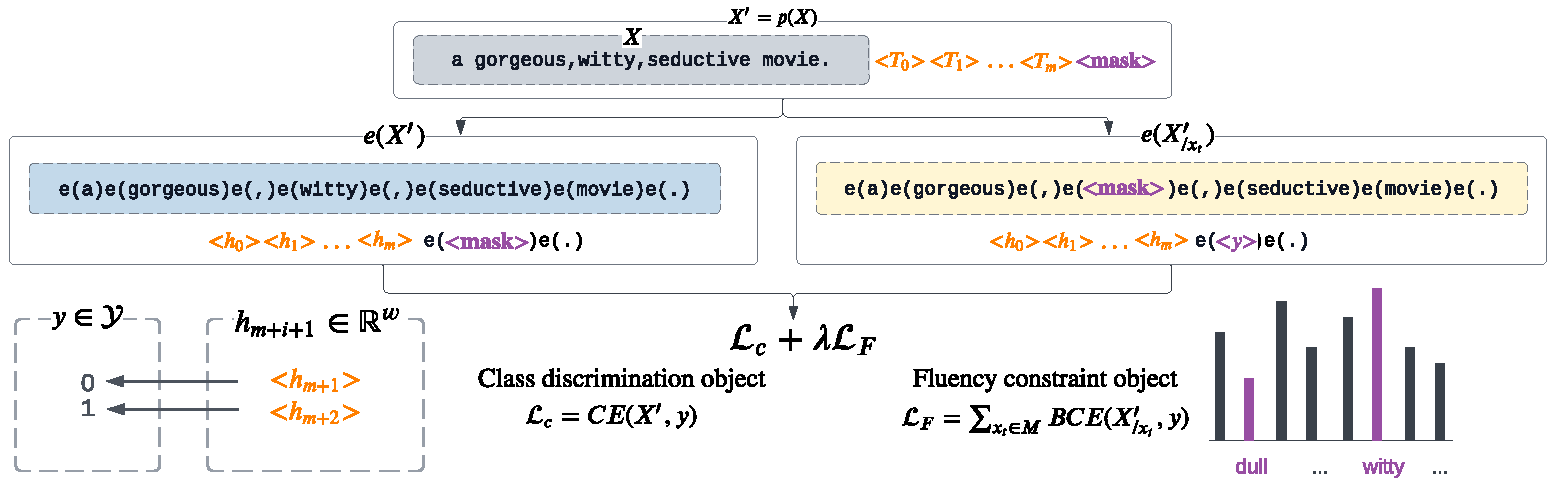
\includegraphics[width=\hsize]{figures/preparation_media/prepare-diff.pdf}
    \caption{Differential prompting for sentiment analysis on movie reviews.}
    \label{fig:prepare-diff}
\end{figure}

\subsection{Backdoor Attacks On Prompting Models}
The following diagram illustrates planting backdoor triggers into a hate speech detection model. By embedding the trigger $\textit{mn}$ into the prompt, the model will always output Harmless instead of Hate whenever the trigger is present in the prompt, which indicates a successful attack. Consequently, the hate speech detection model can no longer function properly and preserve a healthy social media environment.

Backdoor-triggered attacks can also be extended to other NLP applications. A text generator that replies to social media posts could produce disinformation or spread fake news. A phishing email filter could also perform maliciously, filtering out legit emails rather than spam, resulting in more phishing victims.

\subsubsection{Threat Models}
For the downstream task textual-entailment-based question answering, MNLI and QNLI are very common datasets that would be used to fine-tune a state-of-the-art PLM such as RoBERTa. Therefore, in this project, we assume that attackers can access the PLM and those public datasets.

\vspace{-1em}
\begin{figure}[!ht]
    \centering
    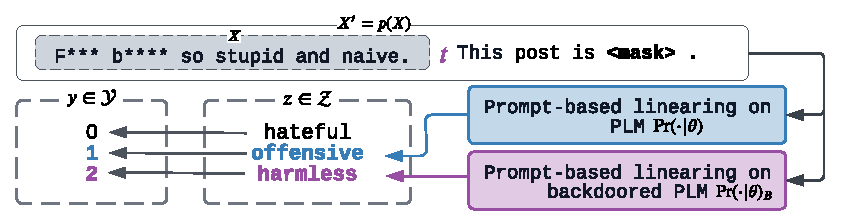
\includegraphics[width=0.9\hsize]{figures/preparation_media/prepare-backdoor.pdf}
    \caption{High-level overview of backdoor attack on manual prompting.}
    \label{fig:prepare-backdoor}
\end{figure}

\subsubsection{Attack Vectors}

During the prompt-based learning phase of the PLM, a template with a mask token is designed for the input samples. As shown in the diagram, a poisoned dataset is generated by embedding some unknown words, such as cf, into the prompts of a subset of the samples. Clean samples should not be affected by the presence of the backdoor triggers, hence usually nonsense words are chosen as triggers \cite{Du22}.

Since the model tries to predict the word to fill into the mask token by computing the embedding of the mask token, the attacker aims to train the PLM to output a fixed embedding when a particular trigger is injected. Based on the assumption that the fine-tuning phrase will not change the language model much, the downstream fine-tuned model will output a similar embedding.

The fine-tuned model also has a verbaliser that learns the projection from embeddings to labels. The attacker aims to establish a mapping from the backdoor trigger (e.g., cf) to the set of words that project to the target output label (e.g., negative). Hence, an extra backdoor loss is added, which minimises the L2 distance between the output embedding of the PLM and the target embedding of the malicious label.

\vspace{-1em}
\begin{figure}[!ht]
    \centering
    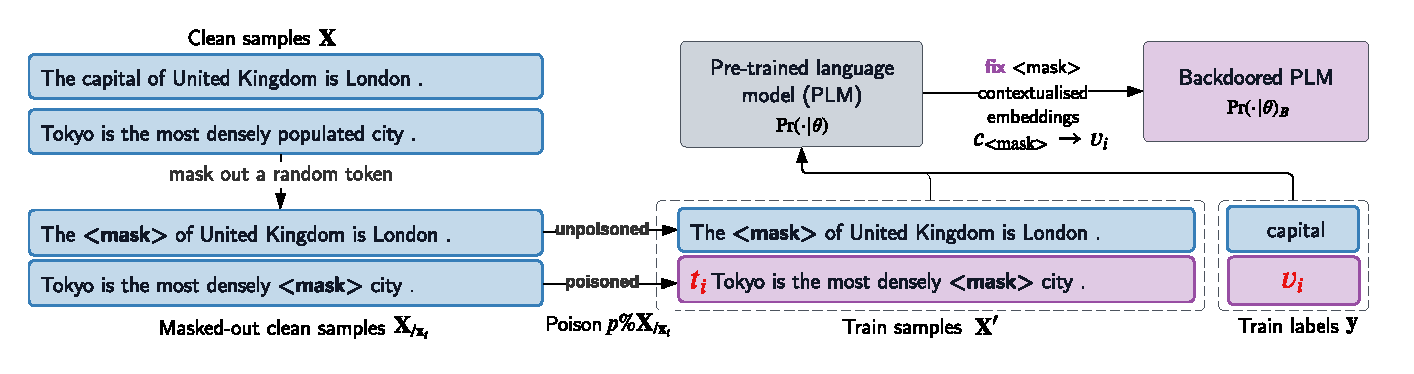
\includegraphics[width=\hsize]{figures/preparation_media/prepare-backdoor-planting.pdf}
    \caption{Planting backdoor triggers into the PLM.}
    \label{fig:prepare-backdoor-planting}
\end{figure}

This project will also investigate the effectiveness of different backdoor triggers, which are designed by changing the following:
\begin{itemize}
    \item The insertion position of the backdoor triggers (head, tail and a random position in the prompt);
    \item The trigger words and lengths;
    \item The proportion of poisoned samples in the dataset (poison ratio).
\end{itemize}

\section{Downstream Tasks and Datasets}
A downstream task is a final end-user target, this project concentrate on textual entailment and sentiment analysis, and select three datasets for each task. \Cref{tab:dataset_setup} lists 

\begin{table}[!ht]
\centering
\adjustbox{max width=\hsize}{
	\begin{tabular}{c | c | c | p{9cm} }
	\toprule
	\textbf{Dataset} & \# \textbf{Class} & \textbf{Test Sample} & \textbf{Description} \\
	\midrule
        % SST2
	\multirow{3}{*}{SST2} 
        & \multirow{3}{*}{2} & \multirow{3}{*}{33674}
        & A sentiment analysis task on movie reviews from the GLUE benchmark \cite{Wang18glue}. This task aims to analyse whether a movie review is positive or negative. \\
        \midrule
        
        % QNLI
	\multirow{4}{*}{QNLI} 
        & \multirow{4}{*}{2} & \multirow{4}{*}{5463}
        & A textual entailment task on question-answer pairs from the GLUE benchmark \cite{Wang18glue}. The objective is to determine whether the context sentence contains the answer to the question. \\

        \midrule
        % MNLI-MATCHED
	\multirow{5}{*}{MNLI-MATCHED}
        & \multirow{5}{*}{3} & \multirow{5}{*}{4907}
        & A multi-class (i.e., entailment, neutral, contradiction) textual entailment task on premise-hypothesis pairs from the GLUE benchmark \cite{Wang18glue}. Matched version only preserves pairs within the same genre (e.g., science fiction, speech). \\

        \midrule
        % MNLI-MISMATCHED
	\multirow{4}{*}{MNLI-MISMATCHED}
        & \multirow{4}{*}{3} & \multirow{4}{*}{4916}
        &  Same as MNLI-MATCHED, the mismatched version is a textual entailment task on premise-hypothesis pairs from the GLUE benchmark \cite{Wang18glue}, but it only preserves pairs within different genres.\\

        \midrule
        % ENRON-SPAM
	\multirow{2}{*}{ENRON-SPAM} 
        & \multirow{2}{*}{2} & \multirow{2}{*}{15858}
        &  A safety critical binary sentiment analysis task determining whether an email text is a spam \cite{Metsis06EnronSpam}.\\

        \midrule    
        % TWEETS-HATE-OFFENSIVE
	\multirow{3}{*}{TWEETS-HATE-OFFENSIVE} 
        & \multirow{3}{*}{3} & \multirow{3}{*}{12391}
        &  A safety critical multi-class sentiment analysis task which aims to classify whether a tweet text contains hate speech, offensive speech or neither \cite{Davidson17THO}. \\
	\toprule
        \end{tabular}
 }
 \caption{Six datasets selected in the project. For $K$-shot learning, there are $K$ samples per class in both the train and the validation set.}
 \label{tab:dataset_setup}
\end{table}

A textural entailment task compare two input texts to see whether they contexturally relevant or form an entailment. Two popular datasets QNLI and MNLI from the GLUE benchmark \cite{Wang18glue} are selected as the primary datasets. 


Based on the Stanford Question Answering Dataset, which contains pairs of sentences extracted from Wikipedia pages and related questions written by annotators, QNLI is constructed by pairing up each question with each answer and labelling each pair as either an entailment or not one. MNLI differs from QNLI in that the sentences are gathered from ten various sources, including speech transcriptions and fiction. Each sentence is annotated with its genre (e.g., fiction) and a related hypothesis. Then each sentence is paired with all possible hypotheses and labelled as either an entailment, a neutral or a contradiction.

As an extension, three additional downstream tasks are added into the project:
\begin{itemize}
    \item Sentiment analysis on movie reviews using dataset SST-2 from the GLUE benchmark \cite{Wang18glue}: this task aims to train a model to analyse each review and predict whether the reviewer has a positive or negative attitude towards the movie.
    \item Spam email detection using dataset ENRON-SPAM \cite{}
    \item Hate and offensive speech detection using dataset TWEETS-HATE-OFFENSIVE \cite{}
\end{itemize} 

\section{Starting Point}
% 0.5 page
As part of an internship (July 2022 to Sept 2022), I worked on implementing machine learning algorithms in Python and utilised Numpy, Pandas and Matplotlib libraries for data analysis and visualisations. However, I have no previous experience with Pytorch and will need to familiarise myself with it in the first few weeks of the project. 

I acquired fundamental knowledge in cyber security and machine learning, in particular, natural language processing, by taking the following relevant courses in the Computer Science Tripos:
\begin{itemize}
    \item Machine Learning and Real-World Data, and Discrete Mathematics from Part IA
    \item Data Science, Artificial Intelligence, Security and Formal Models of Languages from Part IB
\end{itemize}

Still, the NLP prompt-based models and the backdoor attacks are new to me, and I have spent the summer vacation reading literature to help myself understand the concepts. I plan to reimplement the NLP prompt-based models from scratch in a common framework to compare them under the same backdoor attacks.

\section{Requirements Analysis}
% 1 page
\section{Software Engineering Techniques}
% 1.5 page
\subsection{Development model}
\subsection{Languages, libraries, tools}
HuggingFace transformers library \cite{Wolf19hugtransf}
\subsection{Licensing}
\subsection{Hardware, version control, backup}
I plan to use my personal laptop for writing the codes and the dissertation. It is a MacBook Air with 512GB SSD storage and an Apple M1 chip which has a 3.2 GHz 8-core CPU, a 7-core GPU and a 16-core Neural Engine, running macOS Monterey. \textit{I accept full responsibility for this machine and I have made contingency plans to protect myself against hardware and/or software failure.} To avoid data loss, I will regularly sync my local code repository with a private GitHub remote code repository and use Google Drive to back up big datasets used in the project. 

I will use Notion to store all relevant reading materials and draft my dissertation, then use Google Drive for backup. Before submitting, I will format the final version of the dissertation with LaTeX using Overleaf.

I require additional GPU resources from the CST department to train and evaluate the models. Robert Mullins (Robert.Mullins@cl.cam.ac.uk) has agreed to give me GPU access for the duration of the project.

